\documentclass[oneside, fleqn]{book}
\usepackage[utf8]{inputenc}
\usepackage[T1]{polski}
\usepackage{graphicx}
\usepackage{amsmath}
\usepackage{amssymb}
\usepackage{times}
\usepackage{multirow}
\usepackage{tikz}
\usepackage{url}

\title{Święty Mikołaj}
\author{Jakub Ronkiewicz}
\begin{document}
\frontmatter
\maketitle
\tableofcontents % wstawianie spisu tresci
\mainmatter
\chapter{Historia postaci}
\section{Ogólne informacje}
\begin{figure}[hb]
\centering

\includegraphics[width=\textwidth]{1.png}
\caption{Ilustracja Mikołaja}\label{rys:mik:1}
\end{figure}
\noindent
Święty Mikołaj – postać starszego mężczyzny z białą brodą ubranego w czerwony strój, który wedle różnych legend i baśni w okresie świąt Bożego Narodzenia rozwozi dzieciom prezenty saniami ciągniętymi przez zaprzęg reniferów. Według różnych wersji zamieszkuje wraz z grupą elfów Laponię lub biegun północny. Dzięki sprawnej promocji praktycznie zastąpił on w powszechnej świadomości tradycyjny wizerunek świętego Mikołaja, biskupa Miry.\cite{nic} Obecnie powszechna forma tej postaci wywodzi się z kultury brytyjskiej i amerykańskiej, gdzie jest jedną z atrakcji bożonarodzeniowych. W większej części Europy, w tym w Polsce, Mikołajki obchodzone są tradycyjnie 6 grudnia jako wspomnienie świętego Mikołaja, biskupa Miry. Rankiem tego dnia dzieci, które przez cały mijający rok były grzeczne, znajdują prezenty, ukryte pod poduszką, w buciku lub w innym specjalnie przygotowanym w tym celu miejscu (np. w skarpecie).\newpage
\section{Zasady pisowni}
5 maja 2004 Rada Języka Polskiego zaleciła, że pomimo iż nazwę imienia (Mikołaj) lub świętego (św. Mikołaj) piszemy wielką literą, to w znaczeniu postaci przynoszącej prezenty z okazji Bożego Narodzenia należy ją pisać małą literą: święty mikołaj (np. Tata przebrał się za świętego mikołaja). Również małą literą pisze się nazwę obrzędu, jakim są mikołajki\footnote{Rada Języka Polskiego przy Prezydium PAN. Komisja Języka Religijnego: Zasady pisowni słownictwa religijnego. Tarnów: Wydawnictwo BIBLOS, 2004.}
\section{Lokalne odpowiedniki}
W Rosji św. Mikołaj był również otoczony kultem jako patron uciśnionych i skrzywdzonych, ale przejętą z zachodu postać rozdającą dzieciom prezenty nazwano Dziadkiem Mrozem(~\ref{rys:mik:2}), ze względu na podobieństwo do bajkowej postaci nazywanej Moroz Krasnyj Nos. Zgodnie z tradycją, rozdaje on prezenty wraz ze Śnieżynką. W tradycji bizantyńskiej jego odpowiednikiem jest Święty Bazyli, który obdarowuje prezentami dzieci w dniu 1 stycznia. W Wielkopolsce, na Kujawach, na Pałukach, na Kaszubach i na Pomorzu Zachodnim prezenty na Boże Narodzenie tradycyjnie przynosi Gwiazdor, święty Mikołaj przynosi prezenty 6 grudnia. W Małopolsce prezenty pod choinką zostawia Aniołek, natomiast w nocy z 5 na 6 grudnia prezenty przynosi święty Mikołaj. Na Górnym Śląsku i w Czechach prezenty na Boże Narodzenie przynosi Dzieciątko utożsamiane z postacią Jezusa Chrystusa. 6 grudnia prezenty przynosi święty Mikołaj. Na Dolnym Śląsku oraz na Opolszczyźnie prezenty w Boże Narodzenie przynosi Gwiazdka. Mieszkańcom Płaskowyżu Tarnogrodzkiego natomiast na Boże Narodzenie prezenty przynoszą krasnoludki. Mikołaj jedynie 6 grudnia.
\begin{figure}[htbp]

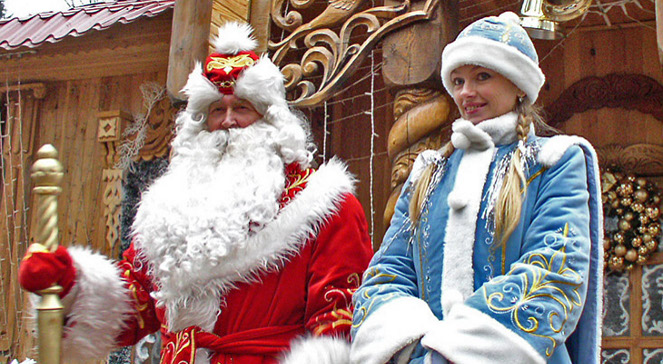
\includegraphics[width=\textwidth]{2.jpg}
\caption{Dziadek Mróz ze Śnieżynką}\label{rys:mik:2}

\end{figure}
\section{Mikołaj obecnie}
Obecny wizerunek – czerwony płaszcz i czapka – został spopularyzowany w 1930 roku przez koncern Coca-Cola, dzięki reklamie napoju stworzonej przez amerykańskiego artystę, Freda Mizena. Na pewno jednak reklama ta pomogła utrwalić w powszechnej świadomości ten kostium świętego. Rok później nowy wizerunek św. Mikołaja przygotował, także na zlecenie Coca-Coli, Haddon Sundblom.
\begin{figure}[htbp]

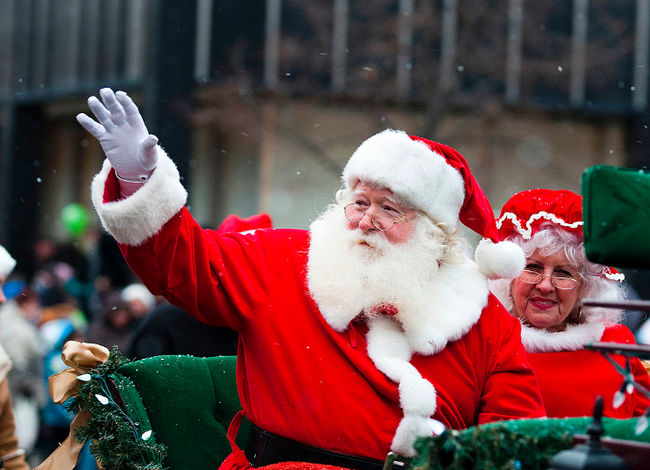
\includegraphics[width=\textwidth]{3.jpg}
\caption{Parada Świętych Mikołajów}\label{rys:mik:3}

\end{figure}

Najbardziej charakterystyczny element stroju świętego Mikołaja – czerwona czapka z białym pomponem, stała się jednym z komercyjnych symboli świąt Bożego Narodzenia.

Współcześnie, ze względów komercyjnych, wizerunek św. Mikołaja jest używany przez handlowców, a okres wręczania prezentów rozciągnął się od imienin Mikołaja do Nowego Roku. Jako postać reklamowa św. Mikołaj jest popularny w okresie świątecznym także w krajach Azji, dokąd trafił z USA. Towarzyszy kończącym rok handlowym promocjom nawet w Chinach, gdzie jest znany jako Staruszek Bożonarodzeniowy
% MATEMATKA
\chapter{Wzory matematyczne}

\paragraph{Świąteczne równanie:} 
\[y=\frac{\ln(\frac{x}{m}-sa)}{r^2} \] \\
Mnożymy obustornnie przez $r^2$: \[ yr^2=ln(\frac{x}{m}-sa) \] \\
Teraz aby zlikwidowac logarytm naturalny, zapiszemy równanie jako potęgi liczby rzeczywistej. Mamy: \[ e^{yr^2} = e^{ln(\frac{x}{m}-sa)} \] \\
Jako, że $e$ i $\ln$ są funkcjami odwrotnymi, jedyne wyrażenie pozostające po prawej stronie równanie to wyrażenie zawarte w nawiasach potęgi. Więc: \[e^{yr^2}=\frac{x}{m}-sa  \] \\
Pozbywamy się ułamków mnożąc przez $m$: \[ me^{yr^2}=x-sam \] \\
Teraz zmieniając zapis $yr^2$ na $rry$ i kolejność mnożenia ( jak wiemy mnożenie jest przemienne ) $sam$ na $mas$, otrzymujemy końcowe równanie: \[ me^{rry}=x-mas \] \\
Wesołych Świąt!

\paragraph{Funkcja kwadratowa}
\begin{displaymath}f(x)=ax^2+bx+c, \textrm{gdzie } a \ne 0\end{displaymath}

\paragraph{Dwumian Newtona}
\begin{displaymath}\binom{n}{k}=\frac{n!}{k\cdot(n-k)!}, \textrm{gdzie } n \ge k\end{displaymath}
\paragraph{Wyznaczenie liczby}
\begin{eqnarray*}
\sum_{k=1}^{n}k(8k^2+2) & = & \sum_{k=1}^{n}(8k^3+2k) = 8\sum_{k=1}^{n}k^3 + 2\sum_{k=1}^{n}k \\
& = & 8\cdot \frac{n^2(n+1)^2}{4} + 2\cdot \frac{n(n+1)}{2} \\
& = & n(n+1)(2n^2+2n+1)
\end{eqnarray*}
\paragraph{Dzielenie wielomianów}
\begin{displaymath}
\begin{array}{lll}
(x^4 - 3x^3 + 3x^2 -4x + 3) & : & (x-1)  =  x^3 - 2x^2 + x -3 \\
\underline{-x^4 + x^3} & &  \\
\qquad -2x^3 + 3x^2 -4x +3 & & \\
\qquad \ \ \underline{2x^3 - 2x^2} & &\\
\qquad \qquad \qquad x^2 - 4x + 3 & & \\
\qquad \qquad \quad \underline{-x^2 + x}  & & \\
\qquad \qquad \qquad \qquad -3x + 3 & & \\
\qquad \qquad \qquad \qquad \ \ \underline{3x - 3} & & \\
\qquad \qquad \qquad \qquad \quad R = 0 & &
\end{array}
\end{displaymath}

\paragraph{Równość funkcji}
\begin{displaymath}
f(x,y) = \frac{x+y}{2} + \frac{|x-y|}{2}, \qquad g(x,y) = \begin{cases} x, &\textrm{gdy } x \ge y\\y, &\textrm{gdy } x < y \end{cases}
\end{displaymath}
% TABELE
\chapter{Tabela, wykres i obrazek}
\section{Tworzymy tabele.}
\begin{table}[htbp]
\begin{tabular}{|c|c|c|c|c|c|}\hline
- & Poniedziałek & Wtorek & Środa & Czwartek & Piątek \\ \hline
8:00 & & & & & \multirow{2}{*}{WdM} \\ \cline{1-5}
9:00 & & & & & \\ \hline
10:00 & & \multirow{2}{*}{WdM} & \multirow{2}{*}{ŚP} & & \multirow{2}{*}{MD} \\ \cline{1-2} \cline{5-5}
11:00 & & & & & \\ \hline
12:00 & \multirow{2}{*}{MD} & \multirow{2}{*}{WdP} & & & \\ \cline{1-1} \cline{4-6}
13:00 & & & & & \multirow{2}{*}{WdM} \\ \cline{1-5}
14:00 & ŚP & & \multirow{2}{*}{WdP} & &  \\ \cline{1-3} \cline{5-6}
15:00 & & & & &  \\ \hline
16:00 & & & \multirow{2}{*}{WdP} & &  \\ \cline{1-3} \cline{5-6}
17:00 & & & & &  \\ \hline
\end{tabular}
\caption{Plan lekcji}
\end{table}


\newpage

\section{Wykres funkcji kwadratowej} 

\begin{figure}[htbp]
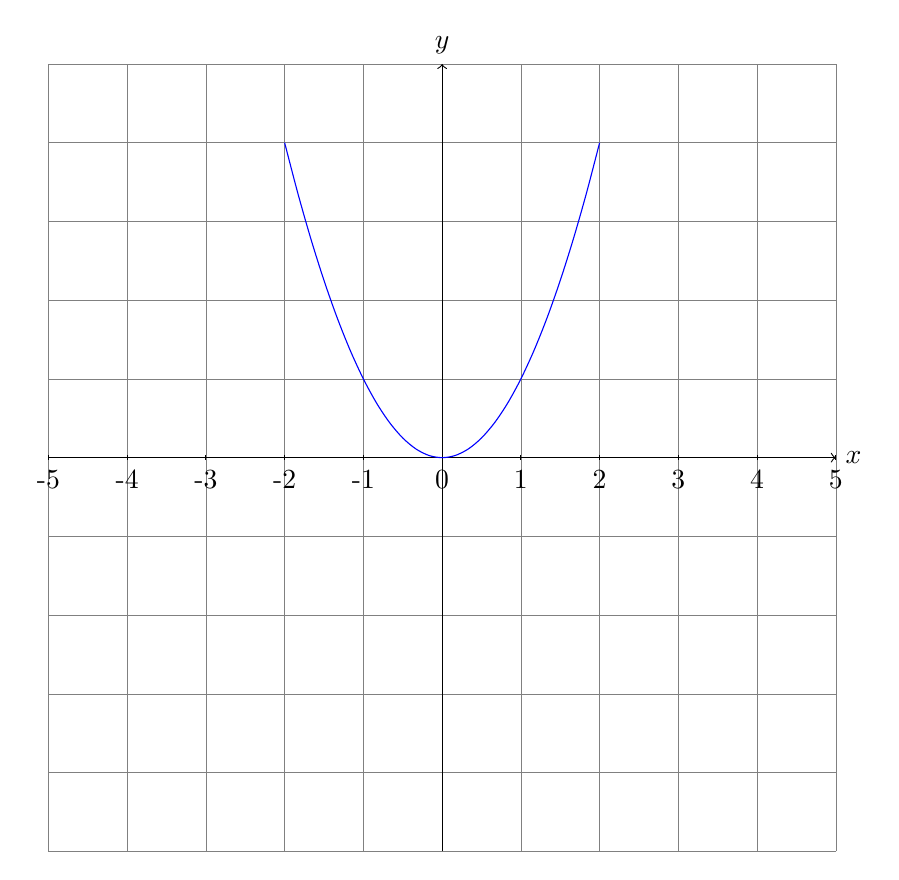
\begin{tikzpicture}
	%kratka
	\draw[gray, very thin, xstep=1, ystep=1] (-5, -5) grid
	(5,5);

	%osie
	\draw[->] (-5,0) -- (5,0) node[right] {$x$};
	\draw[->] (0,-5) -- (0,5) node[above] {$y$};
	%skalowanie osi
	\foreach \x in {-5,...,5}
		\draw (\x, 1pt) -- (\x, -1pt)
			node[anchor=north] {\x};



	\draw[scale=1,domain=-2:2,smooth,variable=\x,blue] plot ({\x},{\x*\x});
\end{tikzpicture}
\caption{Rysowanie funkcji: $f(x)=x^2$ za pomocą Tikz}
\end{figure}

\newpage

\section{Obrazek}
\begin{figure}[htb]
\centering
\setlength{\unitlength}{0.5cm}
\begin{picture}(10,10)
  \put(5,8){\circle{1}}
  \put(5,6.5){\circle{2}}
  \put(5,4.1){\circle{3}}
\end{picture}
\caption{Bałwan}
\end{figure}

\chapter{Cytaty}


\paragraph{Konstanty Ildefons Gałczyński}
\begin{quote}
,,Aby Święta Bożego Narodzenia \\
były Bliskością i Spokojem, \\
a Nowy Rok – Dobrym Czasem.''
\end{quote}

\paragraph{Krzysztof Kamil Baczyński}
\begin{quote}
,,Aniołowie, aniołowie biali,\\
na coście to tak u żłobka\\
czekali, pocoście tak\\
skrzydełkami trzepocąc\\
płatki śniegu rozsypali\\
czarną nocą?''\cite{angel}
\end{quote}

\paragraph{Franciszek Karpiński}
\begin{quote}
,,Bóg się rodzi, moc truchleje,\\
Pan niebiosów obnażony…''\cite{karp}
\end{quote}

\paragraph{ks. Jan Twardowski}
\begin{quote}
,,I pomyśl, jakie to dziwn0e,
że Bóg miał lata dziecinne,
matkę, osiołka, Betlejem.''
\end{quote}

\paragraph{Cyprian Kamil Norwid}
\begin{quote}
,,Przyszła nareszcie chwila ciszy uroczystej,
Stało się – między ludzi wszedł
Mistrz – Wiekuisty''
\end{quote}

\chapter{Tablice matematyczne}
\begin{itemize}
\item  \underline{Średnia arytmetyczna} \\ \\
Średnia arytmetyczna $n$ liczb $a_1,a_2,\dots,a_n$ jest równa: \\
\[ \frac{a_1+a_2+\ldots+a_n}{n} \]
\item \underline{Średnia ważona} \\ \\
Średnia ważona $n$ liczb $a_1,a_2,\dots,a_n$ którym przypisano odpowiednio dodatnie wagi $w_1,w_2.\dots,w_n$ jest równa: \\
\[ \frac{w_1 \cdot a_1 + w_2 \cdot a_2 + \ldots + w_n \cdot a_n}{w_1+w_2+\ldots+w_n} \]
\item  \underline{Średnia geometryczna} \\ \\
Średnia geometryczna $n$ nieujemnych liczb $a_1,a_2,\dots,a_n$ jest równa: \\
\[ \sqrt[n]{a_1 \cdot a_2 \cdot \ldots \cdot a_n} \]
\item  \underline{Średnia harmoniczna} \\ \\
Średnia harmoniczna $n$ dodatnich liczb $a_1,a_2,\dots,a_n$ jest równa: \\
\[ \frac{n}{\frac{1}{a_1}+\frac{1}{a_2}+\ldots+\frac{1}{a_n}}  \]
\item  \underline{Mediana} \\ \\
Medianą uporządkowanego rosnąco ciągu $n$ danych liczbowych $a_1 \le a_2 \le a_3 \le \ldot \le a_n$ jest: \\
\begin{itemize}
\item dla n nieparzystych $a_{\frac{n+1}{2}}$(środkowy wyraz ciągu,
\item dla n parzystych: 
\end{itemize}



\end{itemize}


\backmatter
\begin{thebibliography}{99}\addcontentsline{toc}{section}{Bibliografia}
\bibitem{nic} Nicola Lagioia, \emph{Babbo Natale. Dove si racconta come la Coca-Cola ha plasmato il nostro immaginario Fazi}, 2005, ISBN 88-8112-693-1
\bibitem{arn} Arnaud D'Apremont, \emph{La vera storia di Babbo Natale}, L'Età dell'Acquario, 2005, ISBN 88-7136-224-1
\bibitem{cla}Claude Lévi Strauss, \emph{Babbo Natale giustiziato}, Sellerio, 2002, ISBN 88-389-1190-8
\bibitem{mich}Michael G. Ploog, Babbo Natale. \emph{La leggenda di Santa Claus}, Alessandro, 2001, ISBN 88-8285-099-4
\bibitem{cla}Claudio Corvino, Erberto Petoia, \emph{Storia e leggende di Babbo Natale e della Befana}, Newton Compton, 1999, ISBN 88-8289-314-6
\bibitem{angel}Krzysztof Kamil Baczyński, \emph{Aniołowie Biali}
\bibitem{karp}Franciszek Karpińnski, \emph{Bóg sie rodzi czyli Piesń o Narodzeniu Pańskim}, kolęda polska
\end{thebibliography}
\end{document}
